\section{\absmachine: An abstract machine for programmable switches}
\label{s:absmachine}

% TODO: Say that the atoms can't write to the same packet field.
We present an abstract machine, \textit{\absmachine} that captures several
important features of programmable switch architectures~(\S\ref{ss:abstract})
with deterministic performance. \absmachine is our compiler target throughout
the paper.

\begin{figure*}[!t]
  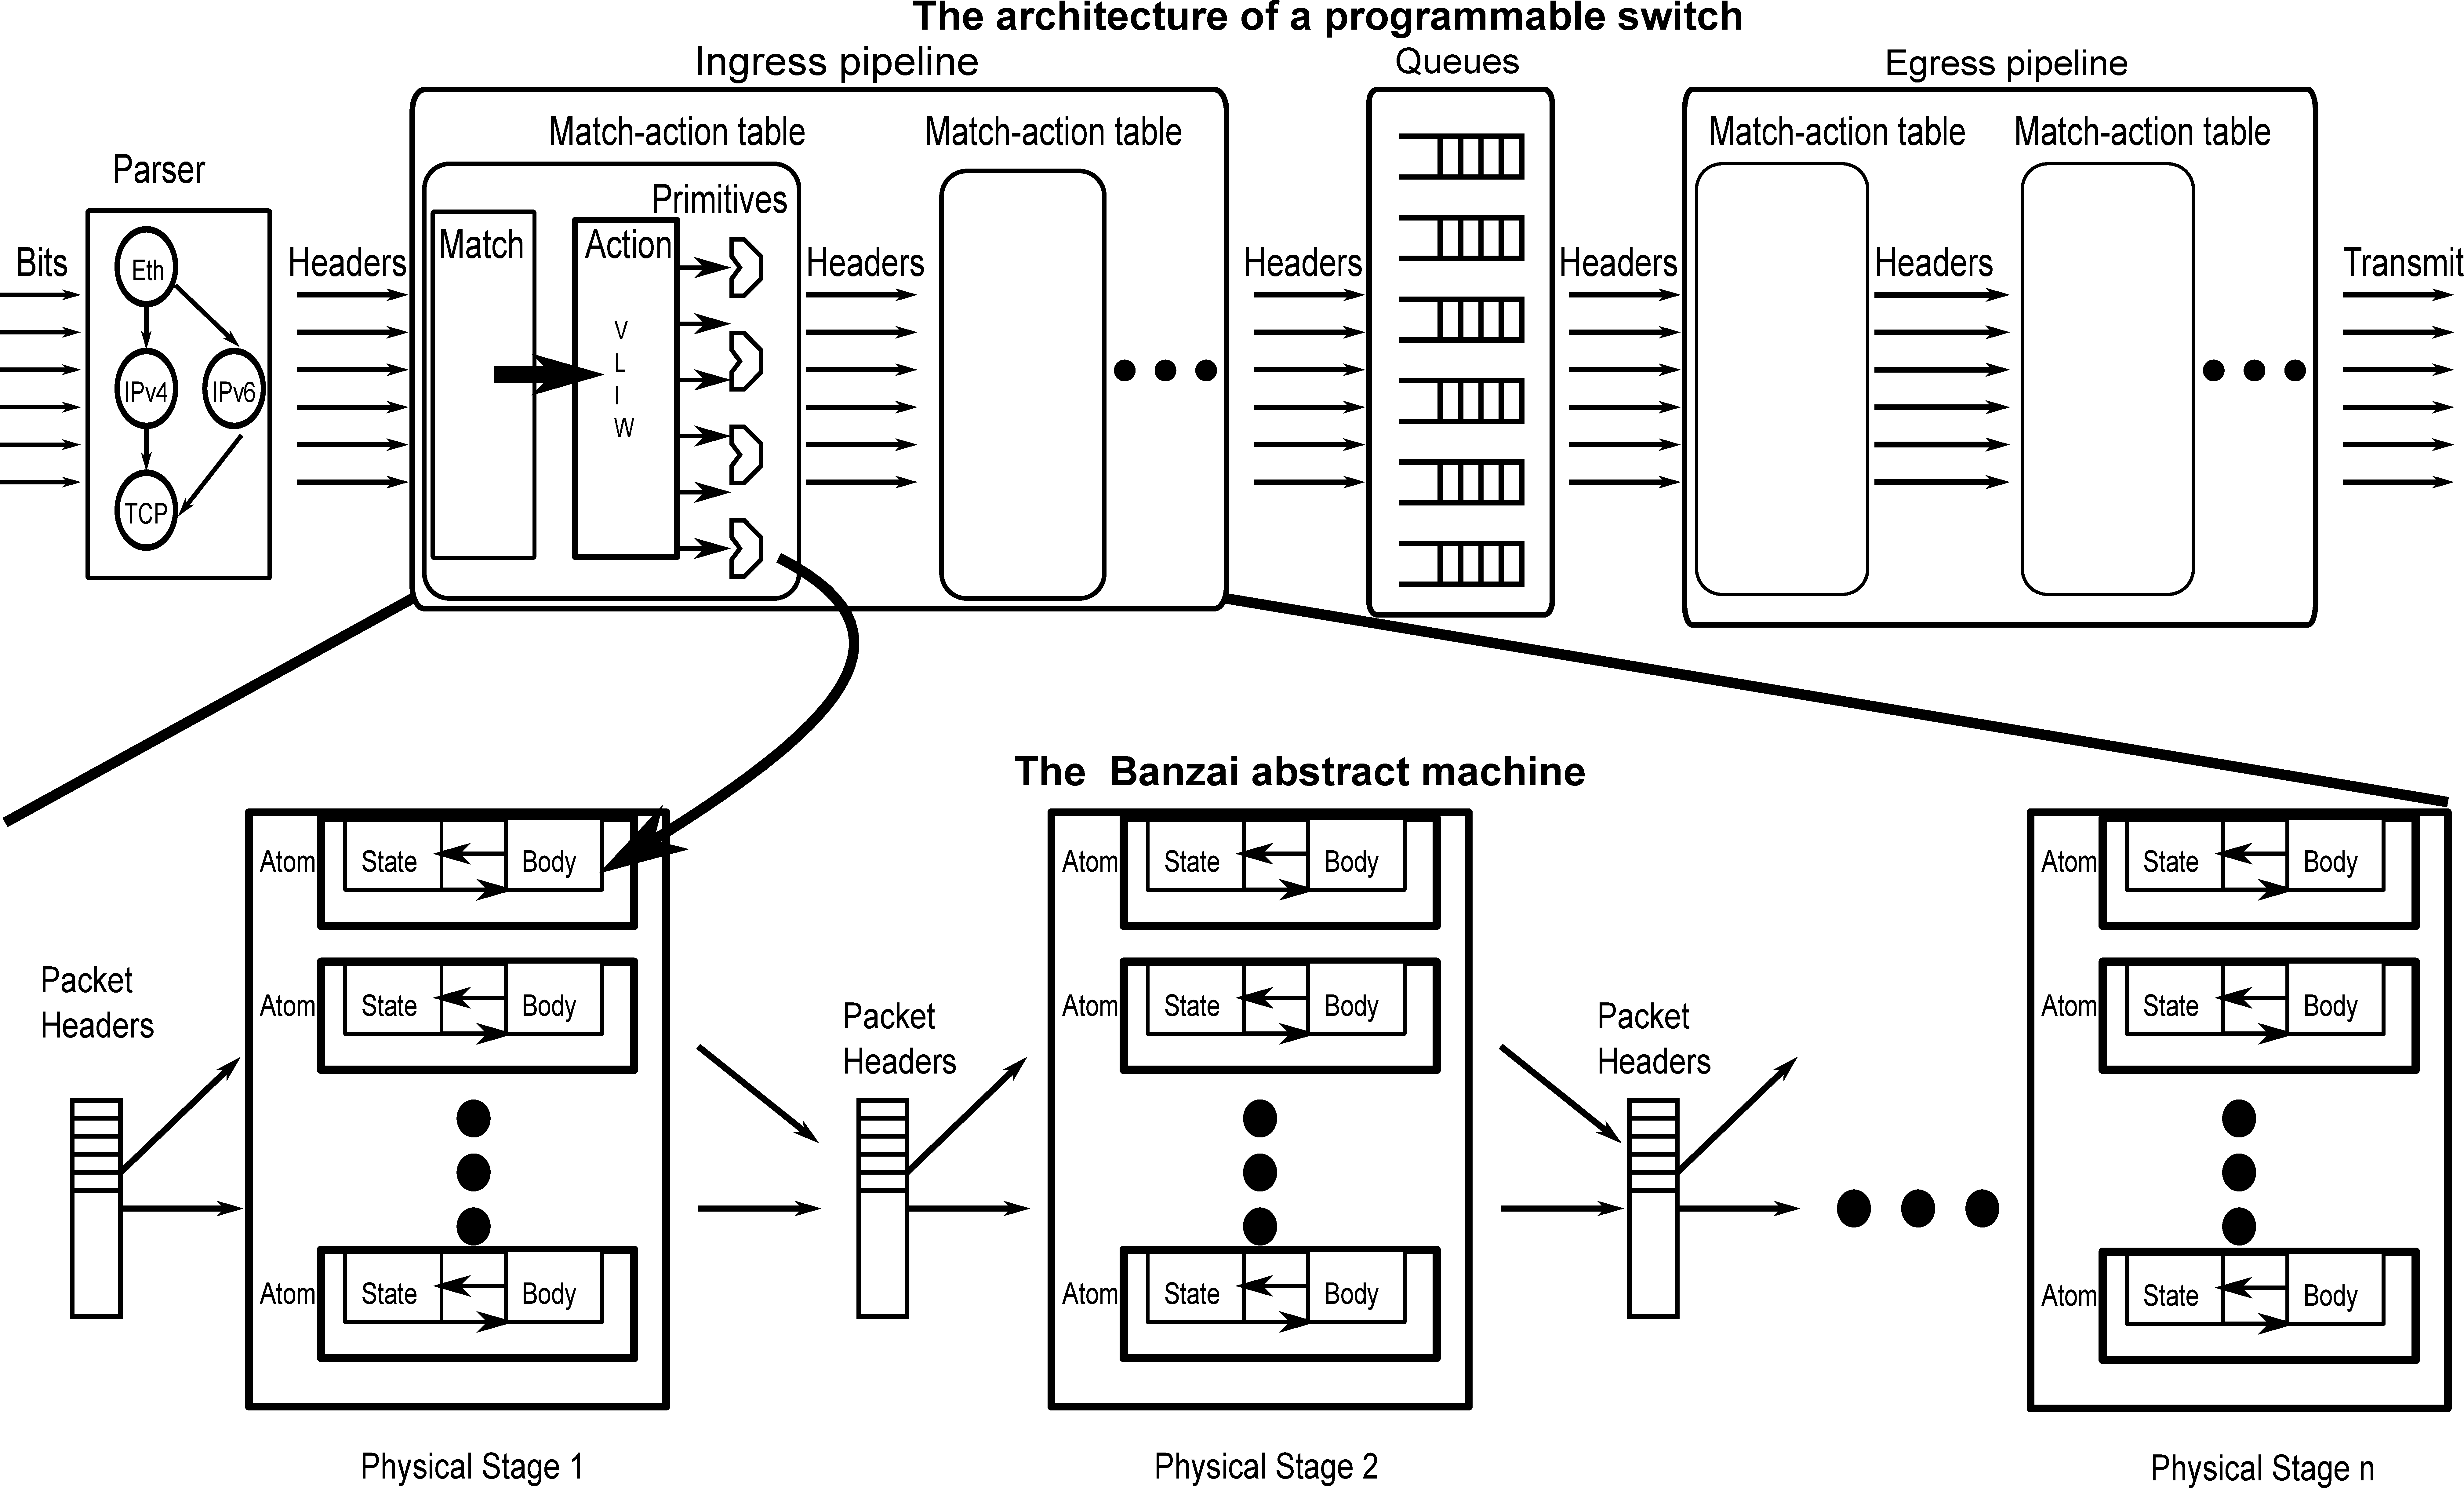
\includegraphics[width=\textwidth]{banzai.pdf}
  \caption{The \absmachine abstract machine and its relationship to programmable switch architectures.}
  \label{fig:switch}
\end{figure*}
Our abstract machine is directly inspired by programmable switch architectures
such as the Reconfigurable Match-Action Table architecture (RMT), Intel's
FlexPipe, and Cavium's XPliant. These architectures assume a switch model
(Figure~\ref{fig:switch}) that consists of an ingress pipeline, followed by the
switch scheduler, followed by an egress pipeline.

\absmachine is an abstract machine that models either of these two pipelines,
with the only difference being the packet fields available at the entrance of
these pipelines. Being an abstract machine, \absmachine only models mechanisms
that are critical to mapping data-plane algorithms. In particular, it models
the computation that happens in each match-action table (i.e. the action half
of the match-action table), but not the match semantics (direct, ternary, or
longest prefix). Notably, \absmachine doesn't model packet parsing.

A switch pipeline in \absmachine has a number of pipeline stages that execute
in parallel with a packet being handed off from one pipeline stage to the next.
Each stage contains a vector of \textit{atoms}, with the atoms themselves
executing in parallel. Informally, an atom is an atomic unit of packet
processing and is represented by a body of imperative code that executes
sequentially. An atom is assumed to complete execution and modify a packet
before the next packet is processed by that atom.

An atom may also contain internal state that can influence the atom's behavior
from one packet to the next and persists across packets. For instance, a switch
counter could be written as an atom as follows\footnote{We use the notation p.x
to represent access to field ``x'' within a packet p and the notation x to
represent access to the state variable ``x'' that persists across packets}.
\begin{verbatim}
  p.tmp     = counter;
  p.tmp2    = p.tmp + 1;
  counter   = p.tmp2;
\end{verbatim}
Similarly, a stateless operation that sets a packet field, such as the
modify\_field action primitive in P4 (equivalently, the bitmasked-set operation
from the RMT architecture) can be written as the atom below:
\begin{verbatim}
  p.field   = value;
\end{verbatim}

The \absmachine abstract machine generalizes several aspects of a programmable
switch architecture. The vector of atoms in each stage generalizes RMT's
very-large instruction-word (VLIW)~\cite{rmt} that executes primitive actions
on independent packet fields in parallel. The presence of internal state in an
atom models persistent switch state residing on a switch such as meters,
counters, , and P4's register abstraction in a unified manner.

\textbf{Constraints on atoms} \\

Any switch hardware running at line rate will need to constrain atoms to bound
the execution latency of each atom and provide deterministic performance. We
impose two such constraints that distinguish \absmachine from software
packet-processing platforms such as Click and Network Processors such as the
Intel IXP, which tradeoff deterministic performance for greater flexibility in
expressing packet processing code.

First, \absmachine is a shared-nothing architecture: state variables are internal to
a particular atom and their values can only be communicated with atoms in
subsequent stages by writing these state variables into packet fields that are
then read downstream.  This restriction reflects the capabilities of most
switches today: building memories that can be simultaneously accessed from
multiple switch stages is technically challenging.

%%To let a stage communicate state information to a predecessor stage upstream,
%%\absmachine allows packets to be cloned and recirculated back into a pipeline,
%%modeling the loopback interfaces found on most switches today.
Second, we constrain the complexity of atom bodies by definining how atoms are
executed. One execution model is an in-order load-store CPU that can execute at
most $N$ instructions sequentially. Another is a configurable combinational
circuit in hardware~\cite{dataflow}, where the circuit limits the space of
feasible computations and needs its control signals to be configured to match
the behavior of the atom.

We use both models in this paper. For stateless atoms that don't modify state,
we constrain atom bodies to consist of only statements that can be represented
as three-instruction codes. Further, we allow exactly one statement in each
atom body. This corresponds to the set of primitive actions available today in
P4/RMT.  For atoms that do modify state, we consider both models
(\S\ref{s:constraints}) and evaluate how atom body constraints affect whether
or not packet-processing code can be mapped onto \absmachine.
